\newprob{1718629065}
{
    % Active physcs p48 q12
    以下為5個不同的核素。
    \ce{^{56}_{25}P}、\ce{^{60}_{26}Q}、\ce{^{60}_{27}R}、\ce{^{58}_{28}S}、\ce{^{60}_{28}T}。
    \begin{parts}
        \part 哪些核素是同一元素的同位素?\zzh{1}
        \part
        \begin{subparts}
            \subpart $R$ 進行$\beta$衰變後會變為哪一個核素?寫 出代表該衰變的方程。 \zzh{2}
            \subpart 衰變後,$R$的質子數目和中子數目會如 何改變? \zzh{2}
        \end{subparts}
        \part 已知(b)部衰變後的子核素會再進行$\gamma$放射。
        \begin{subparts}
            \subpart 寫出代表該$\gamma$放射的方程。\zzh{1}
            \subpart 進行$\gamma$放射的原子核會發生何事?\zzh{1}
        \end{subparts}
    \end{parts}
}{
    \src{Active Physics p48 q12}
    \par{\par\centering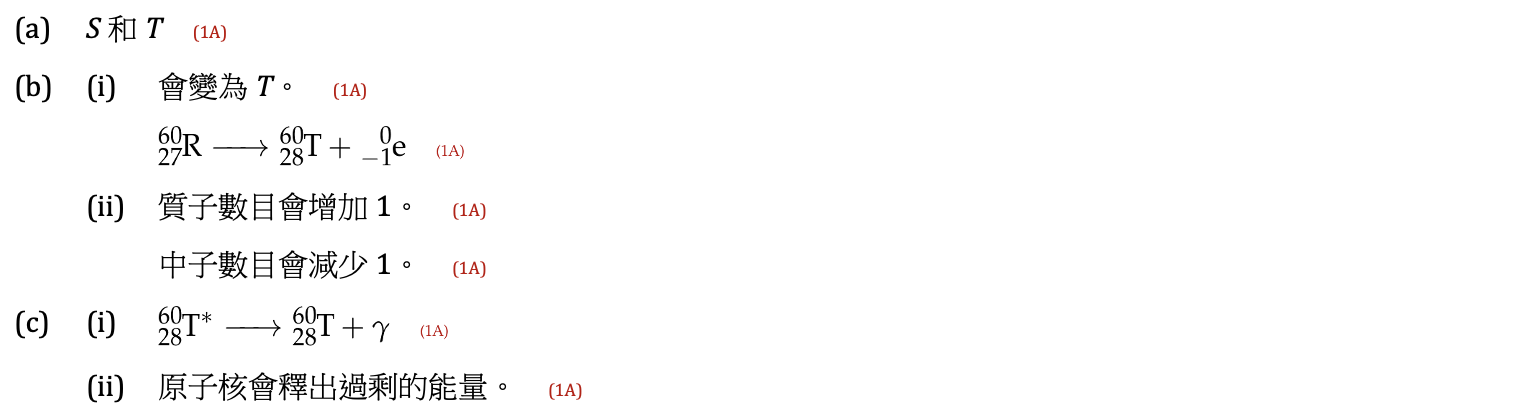
\includegraphics[width=\textwidth]{./img/ch1_prop_lq_2024-06-17-21-57-55.png}\par}
}

\newprob{1718630864}
{
    % Active physcs p48 q13
    圖中顯示元素$A$衰變至元素$F$的一系列衰變過 程。
    \par{\par\centering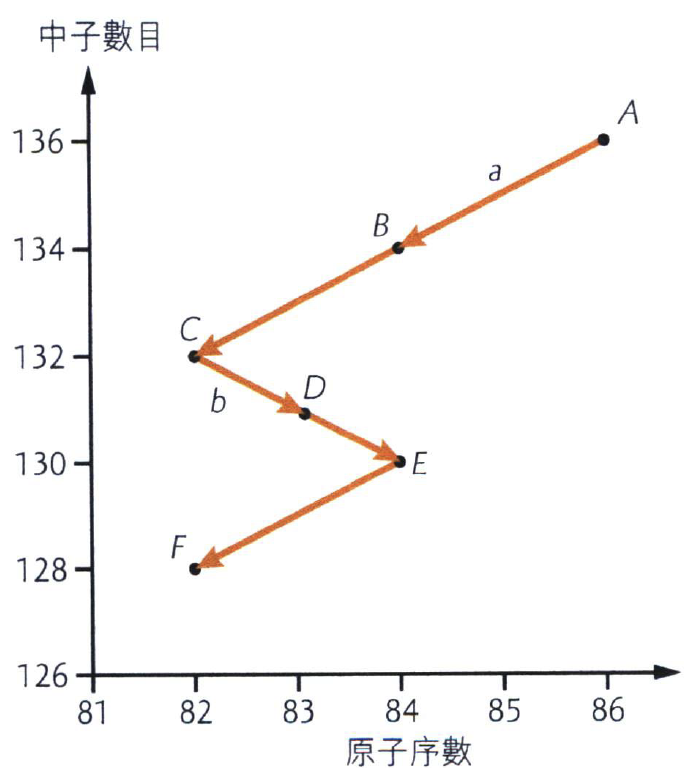
\includegraphics[width=.3\textwidth]{./img/ch1_prop_lq_2024-06-17-21-28-16.png}\par}
    \begin{parts}
        \part 指出過程$a$和$b$分別會放出哪種粒子。\zzh{2}
        \part 求元素 $F$ 的質量數。\zzh{1}
        \part 寫出核方程表示由元素$C$衰變至元素$F$的過 程。 \zzh{2}
        \part 若圖中所示的某個核素會進行$\gamma$放射,我們 可否從該圖中識別出來?試扼要解釋。\zzh{2}
    \end{parts}
}{
    \src{Active Physics p48 q13}
    \par{\par\centering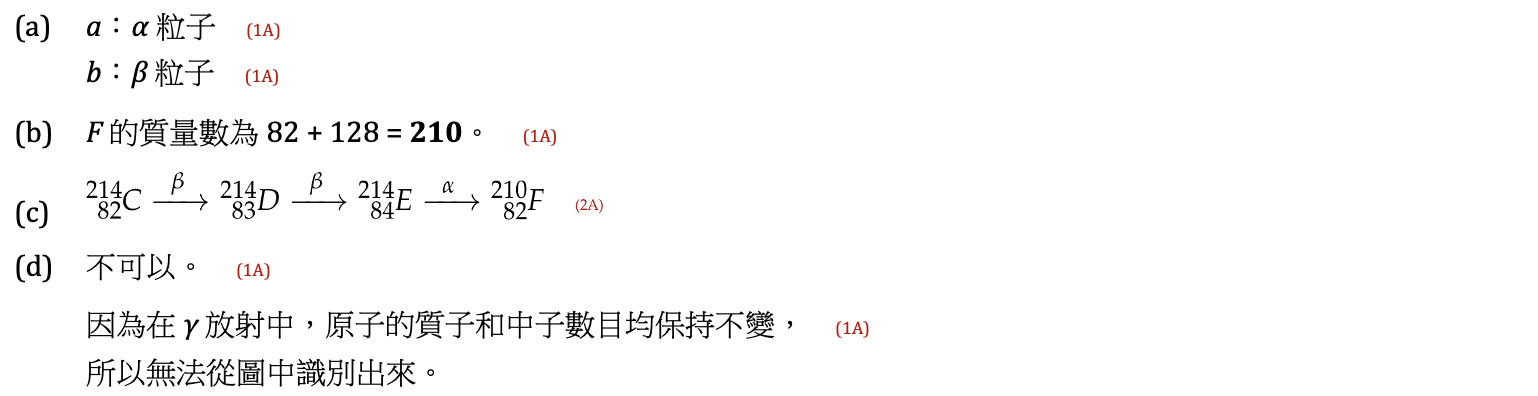
\includegraphics[width=\textwidth]{./img/ch1_prop_lq_2024-06-17-21-58-10.png}\par}
}

\newprob{1718630984}
{
    某學生組裝了下圖所示的電路。把$\alpha$放射源放近 其中一塊金屬板時,氖氣燈泡會發出微弱的燈光。
    \par{\par\centering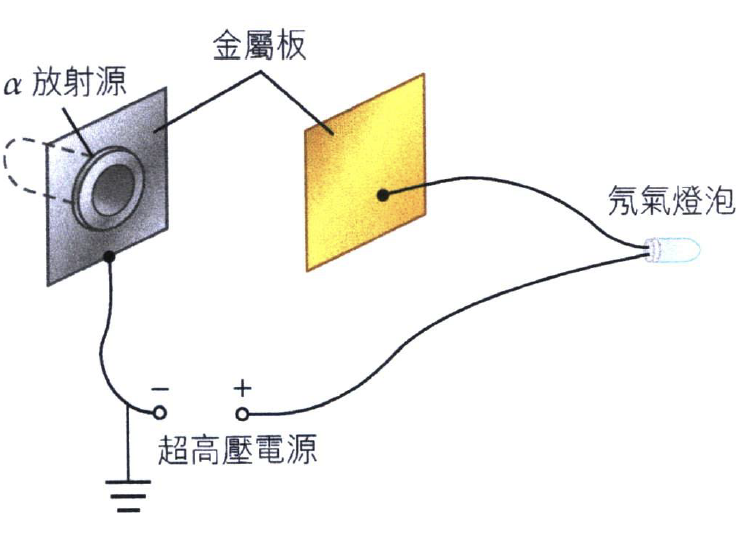
\includegraphics[width=.4\textwidth]{./img/ch1_prop_lq_2024-06-17-21-30-19.png}\par}
    \begin{parts}
        \part 試扼要解釋為何氖氣燈泡會發光。\zzh{2}
        \part 如果一些煙霧粒子飄至兩塊金屬板之間,部 分離子會依附在煙霧粒子上。燈泡會變得更 亮還是更暗?試扼要解釋。 \zzh{2}
        \part 另一名學生認為,由於$\alpha$輻射在空氣中的射 程很短,因此在真空室中進行上述實驗會令 燈泡變得更亮。你同意嗎?試扼要解釋你的 答案。 \zzh{2}
    \end{parts}
}{
    \src{Active Physics p48 q14}
    \par{\par\centering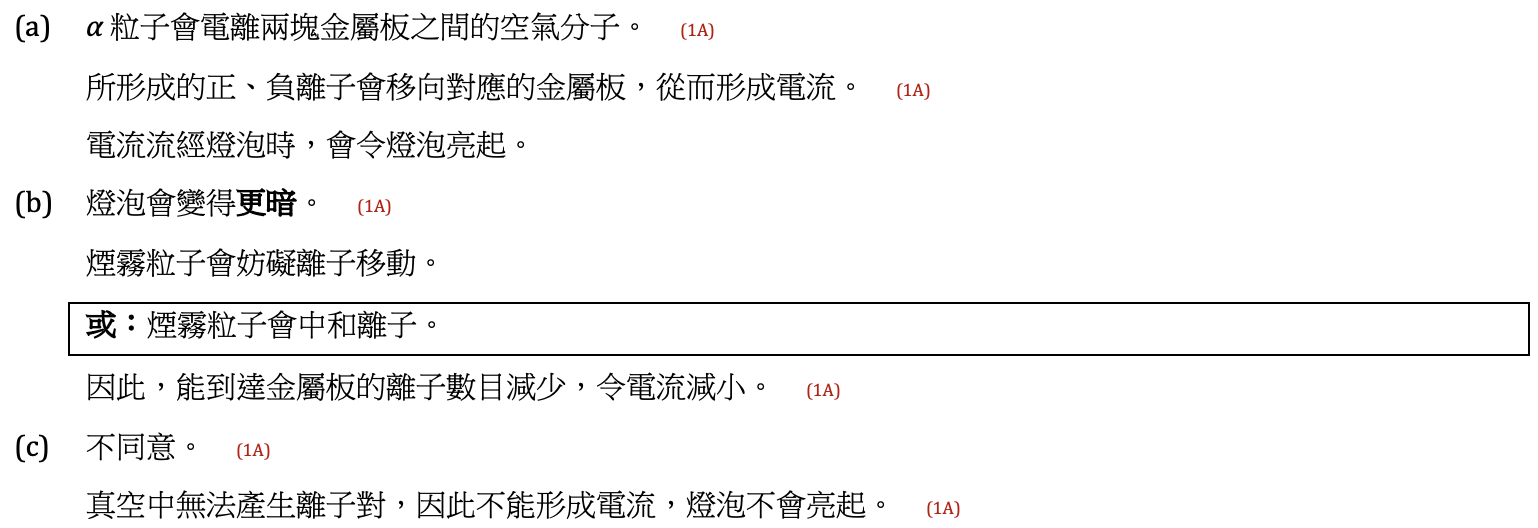
\includegraphics[width=\textwidth]{./img/ch1_prop_lq_2024-06-17-21-58-25.png}\par}
}

\newprob{1718631073}
{
    假設你有圖中所示的儀器。
    \par{\par\centering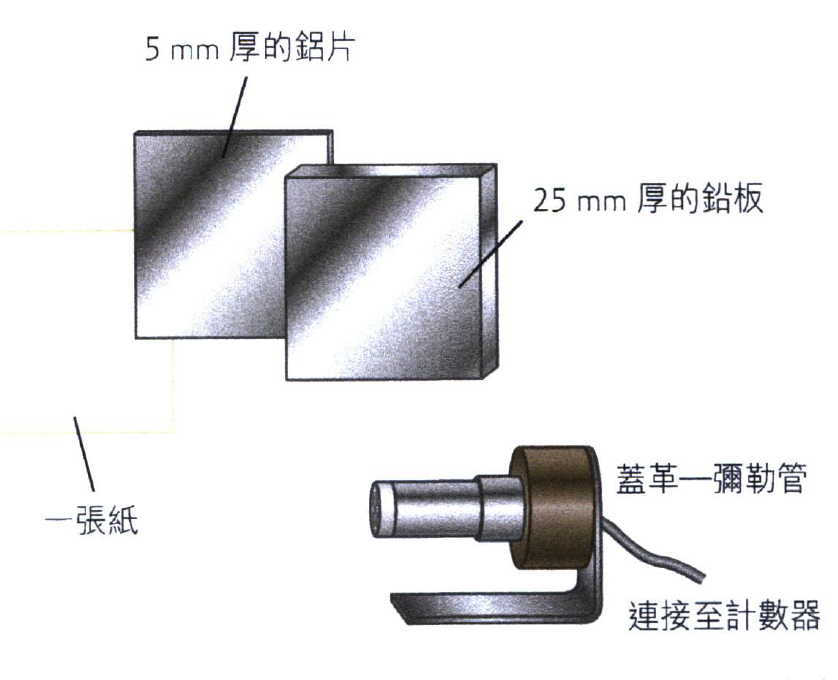
\includegraphics[width=.5\textwidth]{./img/ch1_prop_lq_2024-06-17-21-31-32.png}\par}
    \begin{parts}
        \part 現有一個不明的放射源。試扼要描述你會如 何使用上述的儀器,分辨放射源放出哪種輻 射。 \zzh{4}
        \part 指出另一個方法來分辨放射源所放出的輻射 種類。 \zzh{2}
    \end{parts}
}{
    \src{Active Physics p48 q15}
    \par{\par\centering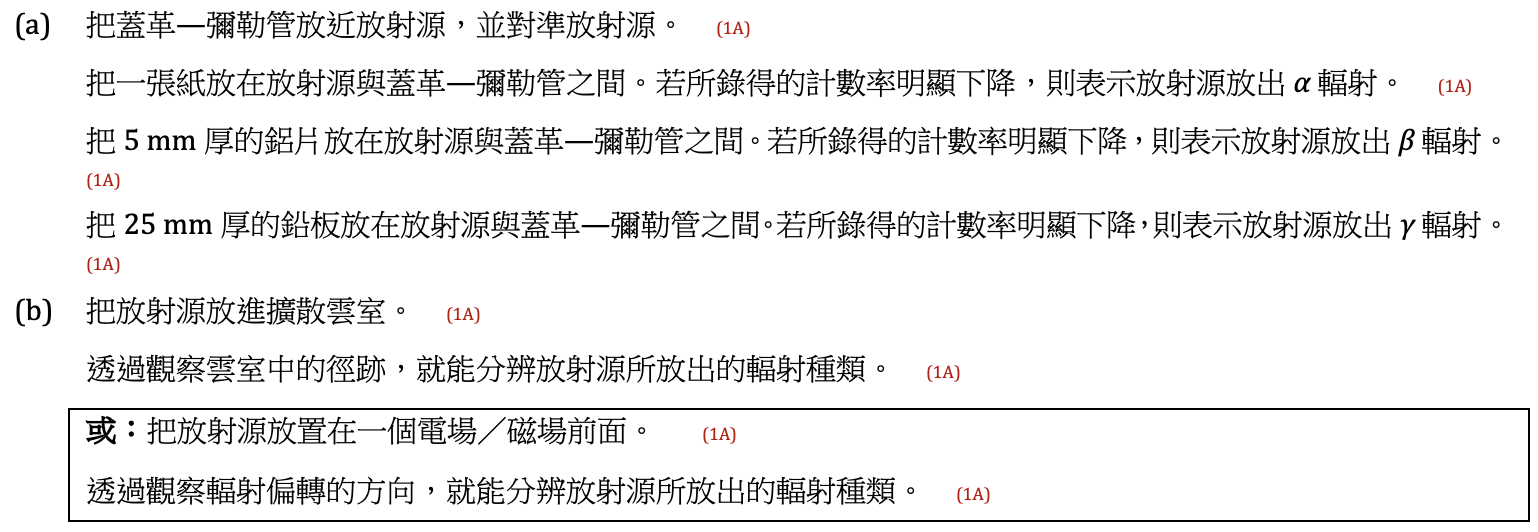
\includegraphics[width=\textwidth]{./img/ch1_prop_lq_2024-06-17-21-58-40.png}\par}
}

\newprob{1718631130}
{
    一名學生進行實驗分辨放射源$X$所放出的輻射種 類。在真空室中,放射源的前方設置了指出紙外 的磁場,磁場的另一端放有攝影底片,如圖。沖 曬底片後,發現底片上有$A$、$B$兩顆黑點。
    \par{\par\centering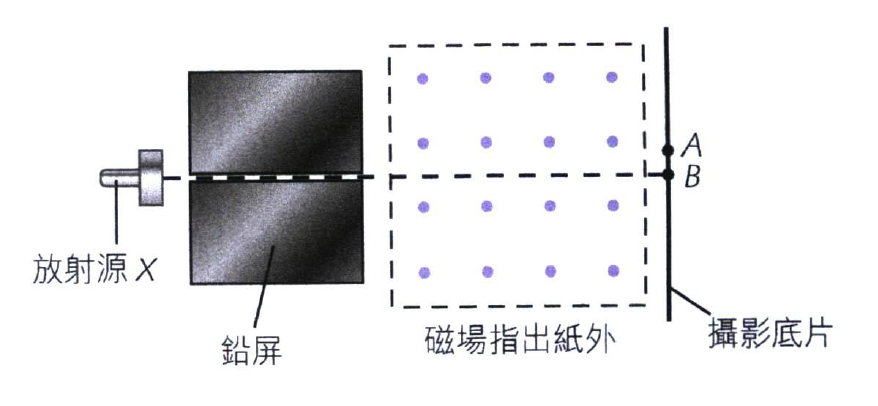
\includegraphics[width=.5\textwidth]{./img/ch1_prop_lq_2024-06-17-21-32-37.png}\par}
    \begin{parts}
        \part
        \begin{subparts}
            \subpart 試扼要解釋鉛屏的功用。\zzh{1}
            \subpart 試扼要解釋為何此實驗必須在真空室中 進行。 \zzh{1}
        \end{subparts}
        \part
        \begin{subparts}
            \subpart 為何根據實驗結果可推斷出放射源會放 出$\beta$輻射? \zzh{2}
            \subpart 國棟認為單憑該實驗結果不足以推斷出 放射源會否放出$\gamma$輻射,原因是黑點$B$ 可能由本底輻射所造成。你同意嗎?為 甚麽? \zzh{2}
        \end{subparts}
        \part 指出另一種探測器,以取代實驗中的攝影 底片。 \zzh{1}
    \end{parts}
}{
    \src{Active Physics p48 q16}
    \par{\par\centering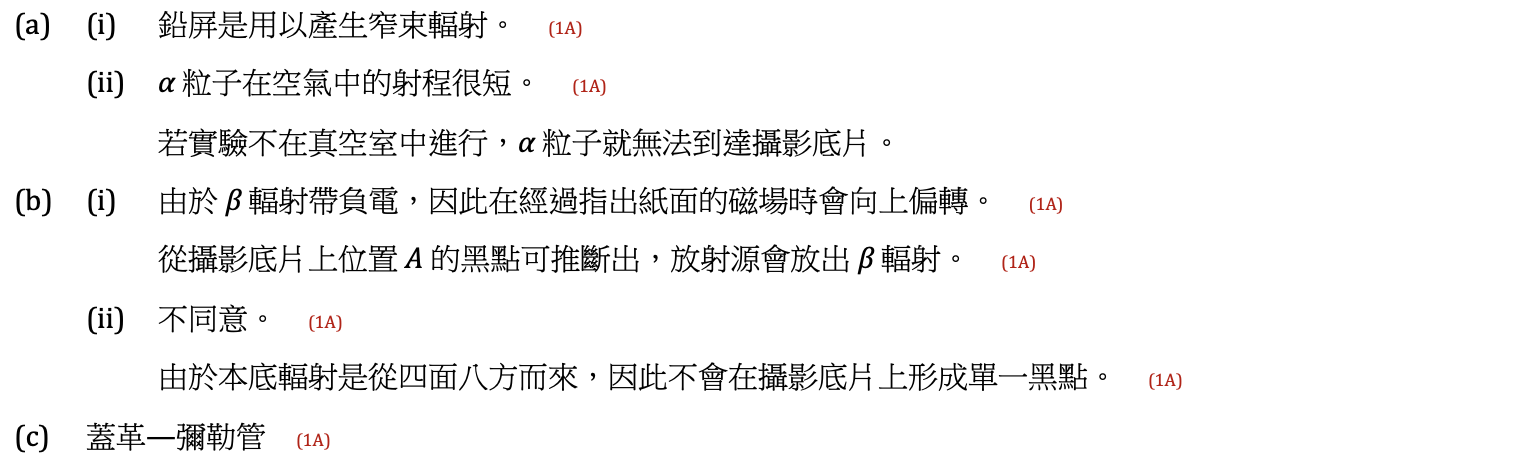
\includegraphics[width=\textwidth]{./img/ch1_prop_lq_2024-06-17-21-59-03.png}\par}
}